	\newpage
\section{Implementacja}		%4
%Wkleić szkielet kodu, wraz z komentarzami. Opisać zmienne, struktury do czego służą. Opisać procedury, metody co wykonują. Opisać nowe zdefiniowane klasy. Opisać dziedziczenie. Opisać nowo utworzone pliki za co odpowiadają.
\textbf{Tworznie Menu:} \newline 
Do stworzenia menu użyty został \textbf{Xamarin.forms Shell}, który zmiejsza złożoność tworzenia aplikacji, oferując podstawowe funkcje. Obejmuje on wspólne środowisko użytkownika nawigacji, schematu nawigacji i zintegrowanej procedury obsługi wyszukiwania.
\newline
\newline
\textbf{Dodawanie strony do menu na przykładzie elementu wyniki:}
\newline
W pliku \textbf{MainPage.xaml}:
\newline
\newline
\begin{figure}[!htb]
	\begin{center}
		\includegraphics[width=12cm]{rys/item.png}
		\caption{Dodanie strony Menu do menu bocznego}
		\label{rys:rysunek012}
	\end{center}
\end{figure}
\newline
, gdzie \textbf{ic\_wyniki} to nazwa ikonki a \textbf{local:Wyniki} to odnośnik do plików strony "Wyniki", które znajdują się w folderze głównym projektu. 
\newline
\newline
\textbf{Dodawanie ikonek do projektu:} \newline
Ikonki pobrane zostały z \textbf{Android Asset Studio} w formacie ".png". \newline
Aby użyć ikonki w projekcie należy umieścić je w dwóch osobnych miejscach. Dla androida jest to folder \textbf{drawable} znajdujący się w folderze resources a dla systemu iOS folder \textbf{resources}.
\newline \newline
\newpage
Działanie menu bocznego w emulatorze Android 8.1:
\begin{figure}[!htb]
	\begin{center}
		\includegraphics[width=6cm]{rys/ZSmenu.png}
		\caption{Widok menu bocznego}
		\label{rys:rysunek013}
	\end{center}
\end{figure}
\newline \newline
\begin{figure}[!htb]
	\begin{center}
		\includegraphics[width=5cm]{rys/ZSotwartastrona.png}
		\caption{Widok strony otwartej po wybraniu danej opcji z menu}
		\label{rys:rysunek014}
	\end{center}
\end{figure}
 \newline
 \textbf{Dodanie pól wyboru na stronie "Wybierz normę":} \newline
 Do stworzenia pól wyboru z których można wybrąć tylko jedną opcję potrzebne jest zainstalowanie pakietu Nuget \textbf{Xamarin.Forms.InputKit}. Przy użyciu tego pakietu można użyć opcji \textbf{RadioButton}, dzięki której tworzona jest lista z polami do wyboru. \newline \newline
 Fragment kodu z pliku \textbf{Wybierz\_norme.xml}: \newline
 \begin{figure}[!htb]
 	\begin{center}
 		\includegraphics[width=12cm]{rys/checkboxy.png}
 		\caption{Dodanie opcji z polami do wyboru}
 		\label{rys:rysunek015}
 	\end{center}
 \end{figure}
 

 \textbf{Dodanie mapy pokazującej obecną lokalizację}
 \newline
 Użycie pakietu Nuget xamarin.forms.maps umożliwia wyświetlenie na stronie mapy ze znacznikiem pokazującym obecną lokalizacje.
 \newline 
 W pliku \textbf{AndroidManifest.xml} w sekcji application - meta-data należy dodać klucz interfejsu API, który można utworzyć na stronie \textbf{developers.google.com}. Wprowadzić należy także nazwe metadanych dla klucza intefejsu API.
 Kolejna linijka również posiada sekcję meta-data i określa numer wersji Google Play usługi. W sekcji uses-library deklarowana jest biblioteka Apache HTTP.

 \begin{figure}[!htb]
 	\begin{center}
 		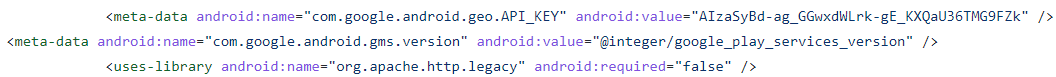
\includegraphics[width=18cm]{rys/map_manifest.png}
 		\caption{Dodanie nowych deklaracji w AndroidManifest.xaml}
 		\label{rys:rysunek016}
 	\end{center}
 \end{figure}
 
 W pliku \textbf{mapa.xaml.cs} utworzona została klasa \textbf{DisplayCurLoc}, w której zawarte są instrukcje odpowiedzialne za wykrycie obecnej lokalizacji.
 \newline
 \newline
 \begin{figure}[!htb]
 	\begin{center}
 		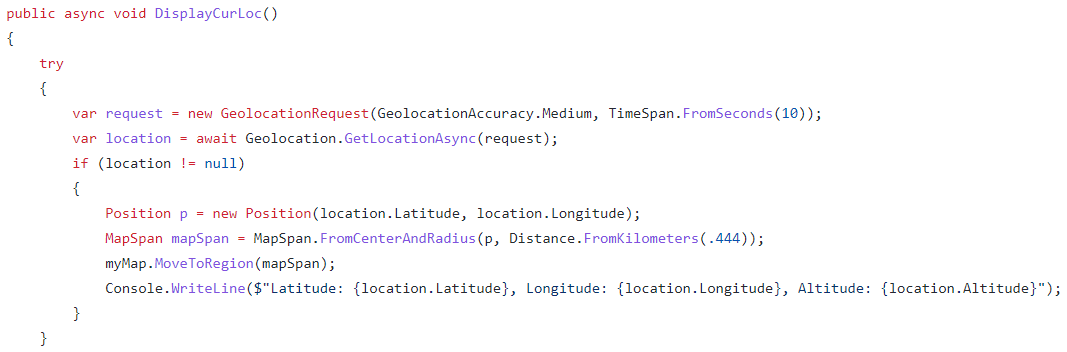
\includegraphics[width=18cm]{rys/mapa_xaml_cs.png}
 		\caption{Dodanie funkcji w mapa.xaml.cs}
 		\label{rys:rysunek017}
 	\end{center}
 \end{figure}
 
 W pliku \textbf{mapa.xaml} wartość opcji IsShowingUser ustawiona jest jako True, dzięki czemu na mapie wyświetlony zostanie znacznik wskazujący na obecną lokalizację. Opcja x:Name nadaje nazwę dla używanej mapy.
 \newline
\begin{figure}[!htb]
	\begin{center}
		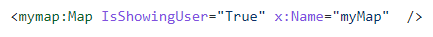
\includegraphics[width=8cm]{rys/mapa_xaml.png}
		\caption{Ustawienie opcji w mapa.xaml}
		\label{rys:rysunek018}
	\end{center}
\end{figure}
   
  


